 \begin{center}\begin{large} Homework 6, Probability theory continued
 \end{large}\end{center}
 \bigskip

\bigskip

\tableofcontents

% 1
\section{Pencils in the boxes}
There are two boxes containing $\{5, 11, 8\}$ and $\{10, 8, 6\}$ white, black, red pencils respectively. One pencil is drawn from each box. What is the probability that the pencils have the same color?

% 2
\section{Questions on exam}
Suppose that you know the answers to 20 questions out of the total 25
questions in the entrance examination, from which you are only asked
3 random questions. What is the probability that you answer all of
the questions?

% 3
\section{Balls in a box}
There are two boxes containing {5, 11} and {10, 8} white, black balls
respectively. First, we take out a ball from each of the boxes. Then, we randomly choose one of them. What is the probability that the
final ball is white?

% 4
\section{Balls in a box (performing steps in order)}
There are three boxes having 4 white and 6 black balls in each of them.
Suppose we perform the following steps in the given order:
    \begin{enumerate}
        \item[a) ] take out a ball from the first box and put it into the second one,
        \item[b) ] take out a ball from the second box and put it into the third one,
        \item[c) ] take out a ball from the third box and put it into the first one.
    \end{enumerate}
    What is the probability of taking a white ball from the third box (after doing \textit{a)-c)})?


% 5
\section{Weapon producing factory}
Two factories produce similar weapons and deliver it to the army warehouse. The first factory’s productivity is two times more than that of
the second one. Moreover, $40\%$ of the weapons produced by the first
factory have some defects, while the same indicator is only $16\%$ for
the second factory. We randomly take a weapon from the warehouse,
test it and it appears to have no defects. What is the probability that
the weapon was produced by the first factory?

% 6
\section{Color-blind person's gender}
According to some statistics, $5\%$ of all males and $0.25\%$ of all females
are color-blind. Assuming that the populations of males and females
are equal, what is the probability that a randomly chosen color-blind person is a male?

% 7
\section{Late for work}
Nune uses her car $30\%$ of the time, walks $30\%$ of the time and rides the bus $40\%$ of the time as she goes to work. She is late $10\%$ of the time when she walks, $3\%$ of the time when she drives, and $7\%$ of the time she takes the bus.

\begin{enumerate}
\item[a) ] What is the probability she took the bus if she was late?

\item[b) ] What is the probability she walked if she is on time?
\end{enumerate}


% 8 
\section{Traffic light}
On the way to the ACA, your
bus passes through a traffic light. The light cycle of the traffic light is $20$
seconds red, $5$ seconds yellow, and $50$ seconds green. What is the
probability that you will pass under a green light?

% 9
\section{Camera film}
After a trip to Garni-Geghard, you bring your camera film to a photography shop. Unfortunately, the shop ruins $4$ photos in a row from your roll which contains $24$ photos. What is the probability that the ruined photos included the
\begin{enumerate}
    \item[a) ] eighth, ninth or tenth photos,
    \item[b) ] eighth, ninth and tenth photos
\end{enumerate}
on the roll (the photos of the Garni Temple)?

% 10
\section{Meeting at shopping center}
Anush and Nairi are shopping at the mall. They agree to split up for a time and then meet for lunch. They plan to meet in
front of Kinopark between 12:00 and 13:00. The one who arrives first agrees to wait $15$ minutes for the other to arrive. After $15$
minutes, that person will leave and continue shopping. What is the probability that they will meet if each one of them arrives at any time between 12:00 and 13:00?

\textit{Hint: Try to represent the problem on coordinate system, by letting
$x$ denote the time Anush arrives, and $y$, the time Nairi arrives.}

% 11 
\section{Triangle formed by line segments}
A line segment is $8$ cm long. Two points are put on the segment at
random locations. What is the probability that the three segments formed by
the two points can make a triangle?

% 12
\section{Unusual rolling die}
Vahe added a dot on the   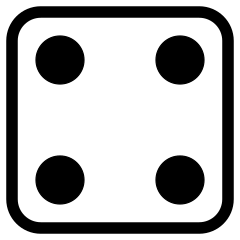
\includegraphics[height=0.9em]{figs/4.png} side of the die, making it 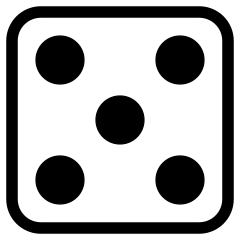
\includegraphics[height=0.9em]{figs/5.png}, and then added two dots on the 
\includegraphics[height=0.9em]{figs/1.png} side, making it 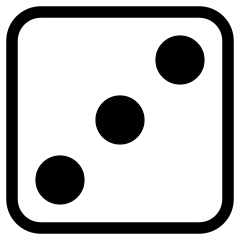
\includegraphics[height=0.9em]{figs/3.png}.
What is the probability that the outcome of the die is greater than $4$? Find the expectation and variance of the die.

% 13
\section{PDF of an RV}
Let $X$ be a random variable with the PDF:
\[
f(x) = \begin{cases}
   2x, & 0 \le x \le 1 \\
   0, & \text{otherwise}
\end{cases}
\]

Find the expectation and variance of
\begin{enumerate}
   \item[a) ] $X$,
   \item[b) ] $2X$,
   \item[c) ] $2X + 7$. 
   
\end{enumerate}